\section{Implementation overview}

The control system outlined in \ref{chap:design} was implemented and simulated in \textit{Matlab R2023b}\cite{MATLAB}. The implementation consists of both Matlab scripts and a Simulink model. The scripts define initial values and fetch all the data the Simulink model requires to run. The interaction is highlighted in\ref{fig:system_arch_flowchart}.

To create the simulation the following models had to be implemented in Simulink:
\begin{itemize}
    \item \textit{Load Forecaster}
    \item \textit{Production Forecaster}
    \item \textit{Battery Module}
    \item \textit{Optimizer}
    \item \textit{Controller}
    \item \textit{Controller Current Control System}
\end{itemize}

\begin{figure}
    \centering
    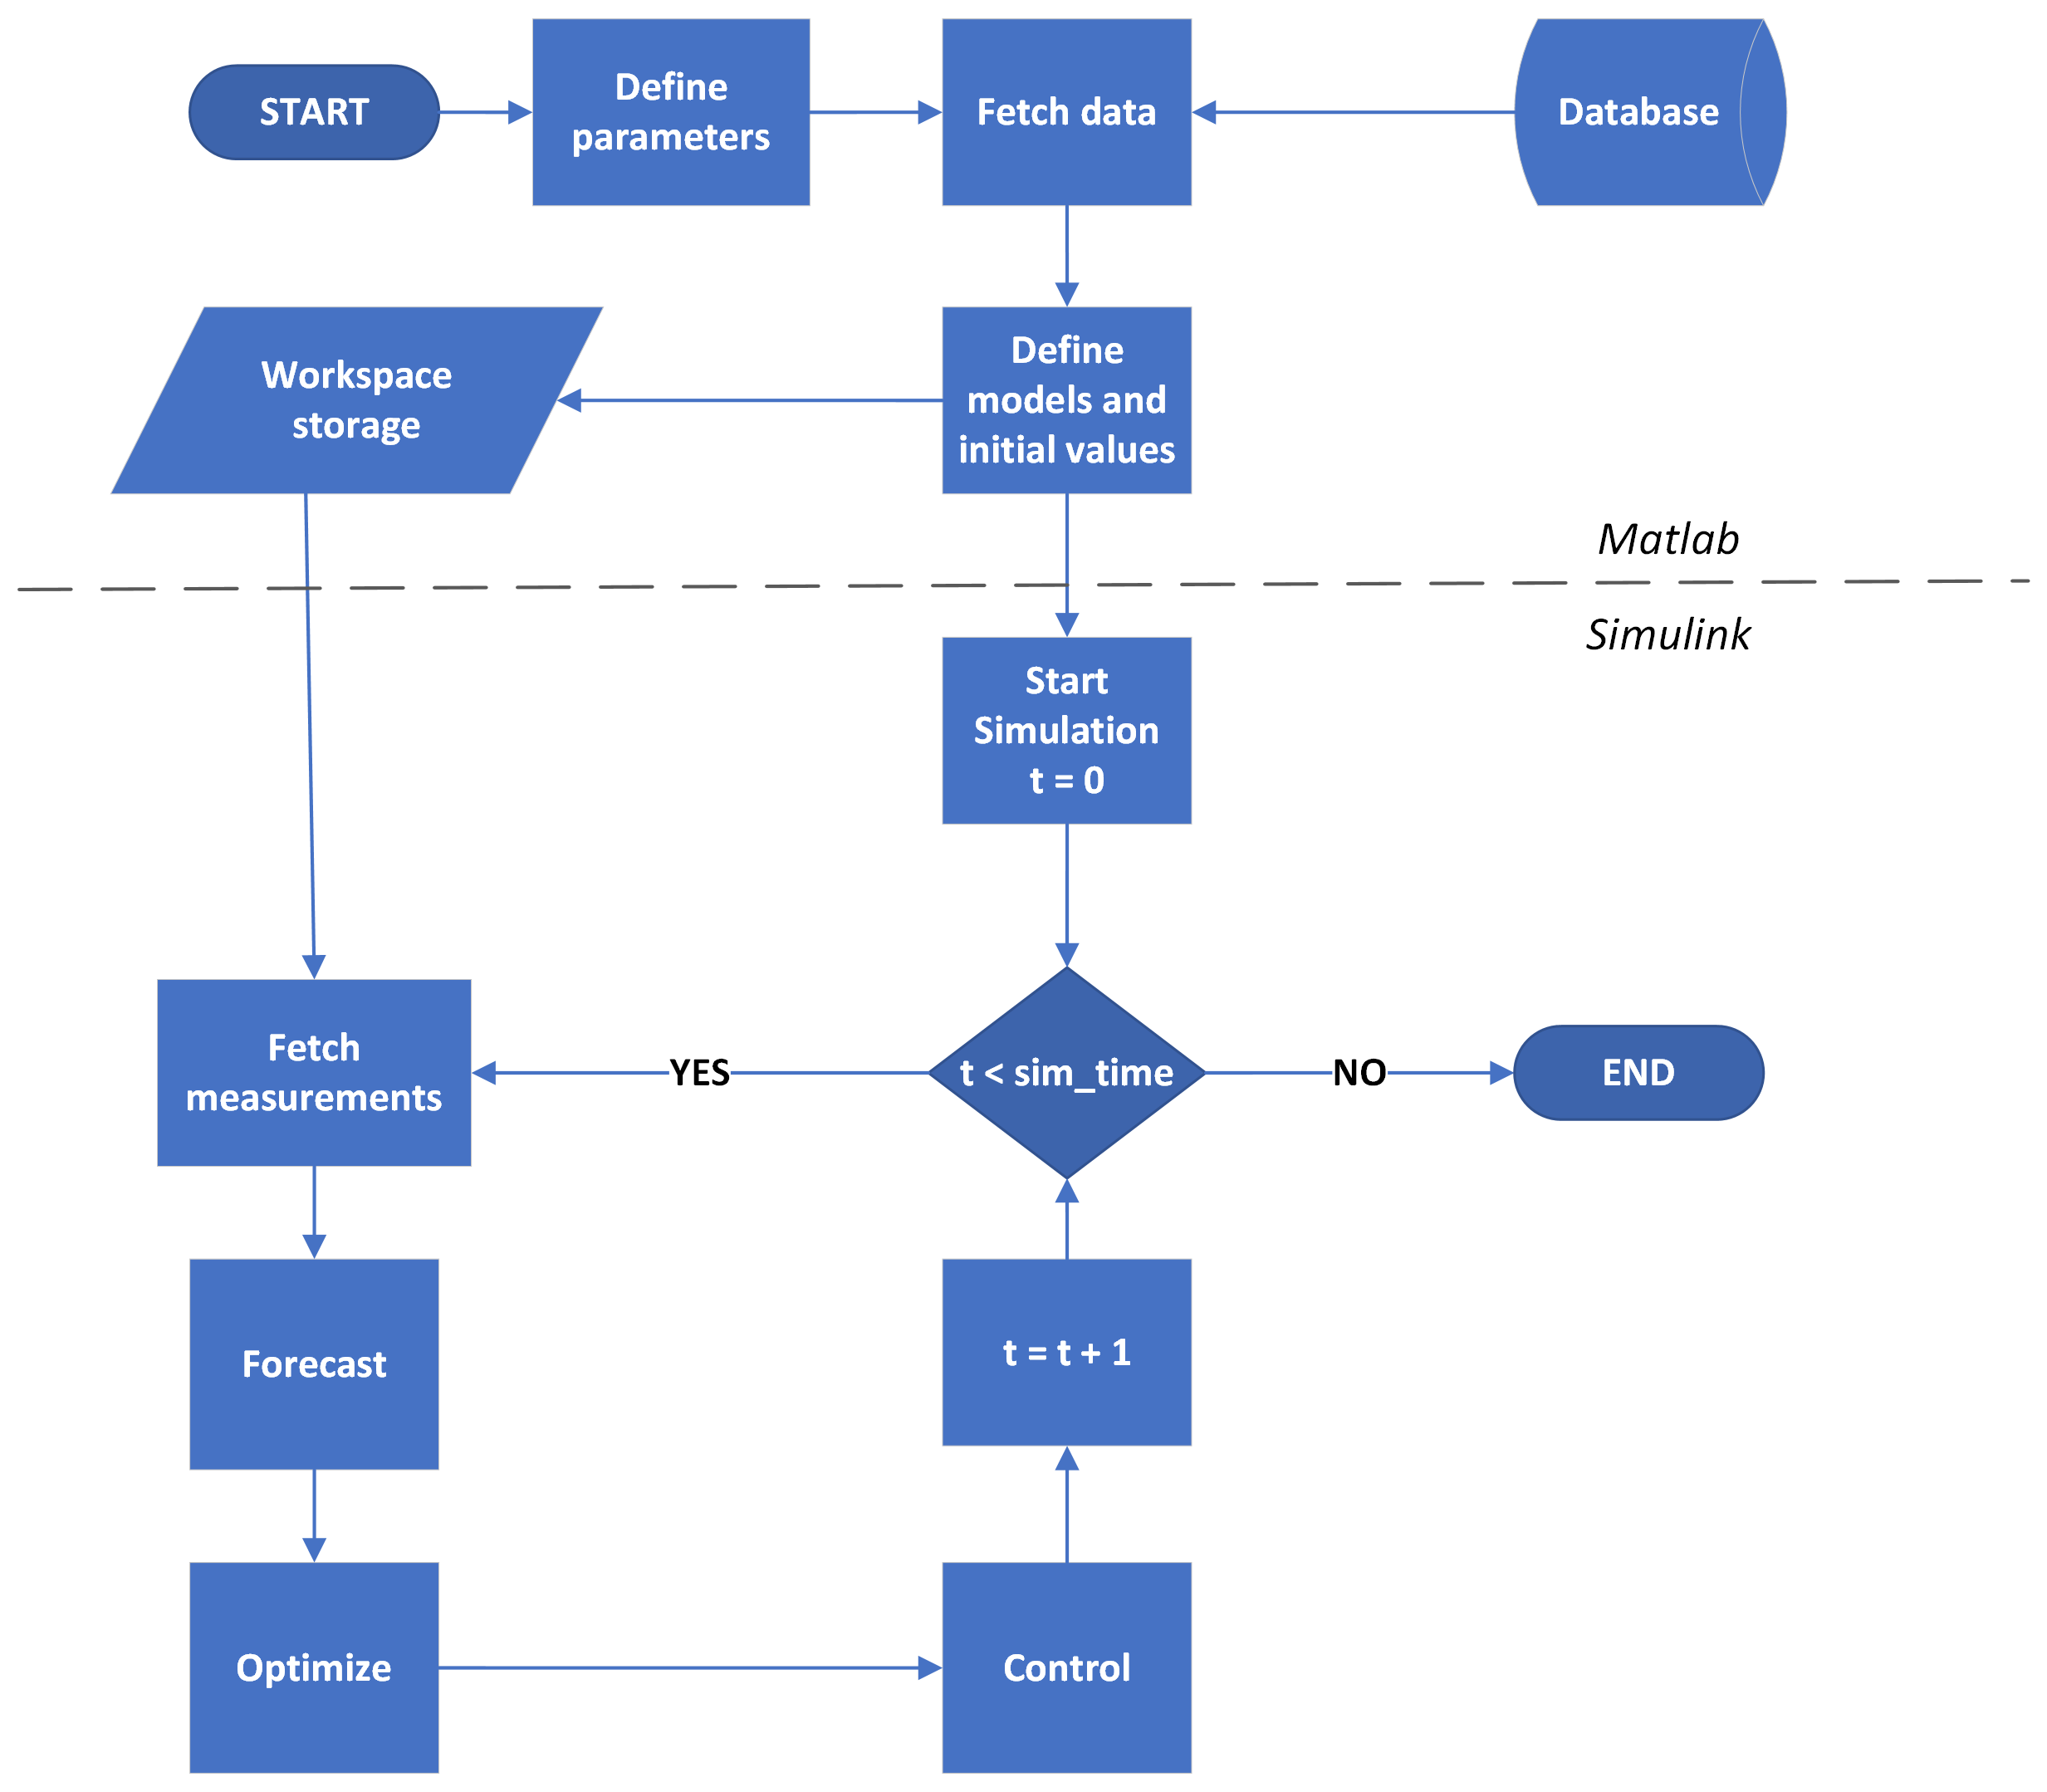
\includegraphics[width=\textwidth]{Figures/08Implementation/system_arch_flowchart.png}
    \caption[Control System architecture flowchart]{Flowchart of the control system architecture.}
    \label{fig:system_arch_flowchart}
\end{figure}


The interaction between the modules is shown in \ref{fig:control_system_block_chart}.

In the implementation, consumption data was collected with a \textbf{15-minute} resolution, however, as production and weather data is in \textbf{1-hour} resolution, and to increase simulation speed, the optimizer is set to run only at every hour. 

\begin{figure}
    \centering
    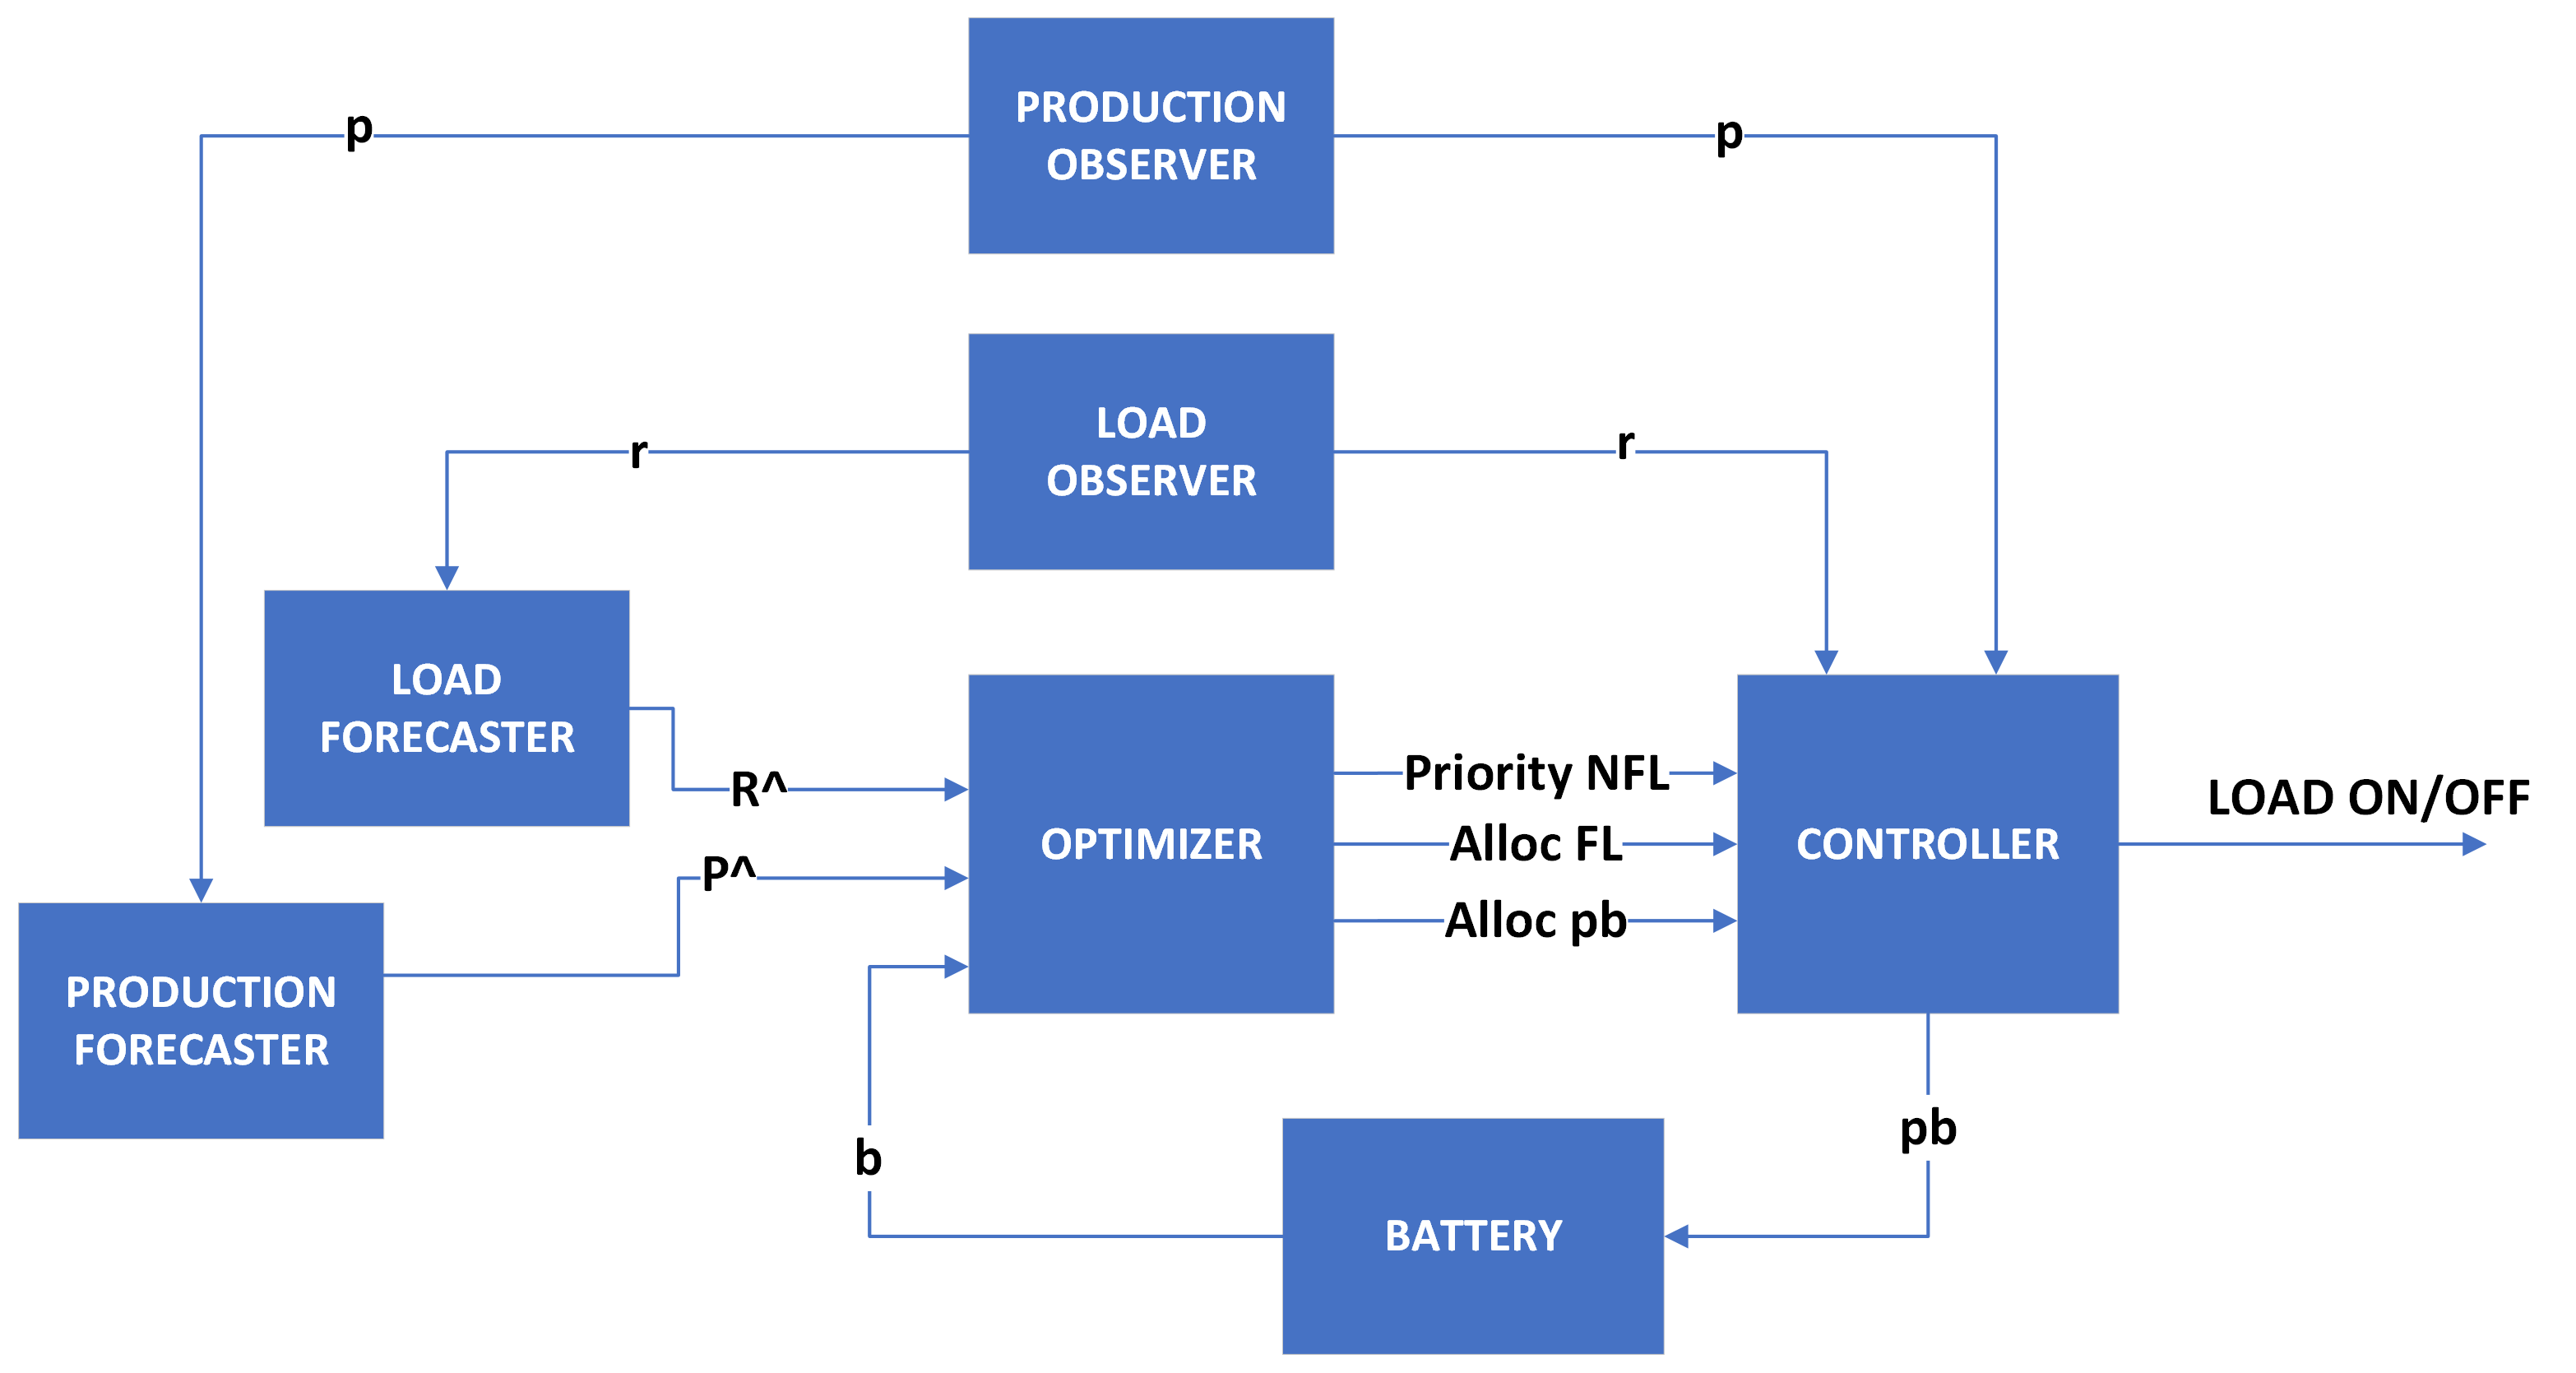
\includegraphics[width=\textwidth]{Figures/08Implementation/control_system_overview.png}
    \caption[Proposed control system block chart]{Chart showing the main components and signals of the implemented solution in simulation. ($p$ - production at ts, $r$ - demand at ts, $\hat{R}$ - demand forecast for the whole prediction horizon. $\hat{P}$ - production forecast for the whole prediction horizon. $p_b$ - power to/from battery, $b$ - battery capacity at ts, Priority NFL - The internal priority of the non-flexible loads, Alloc FL - The power allocated to the flexible loads, Alloc pb - allocated power to/from the battery.)}
    \label{fig:control_system_block_chart}
\end{figure}

\begin{figure}
    \centering
    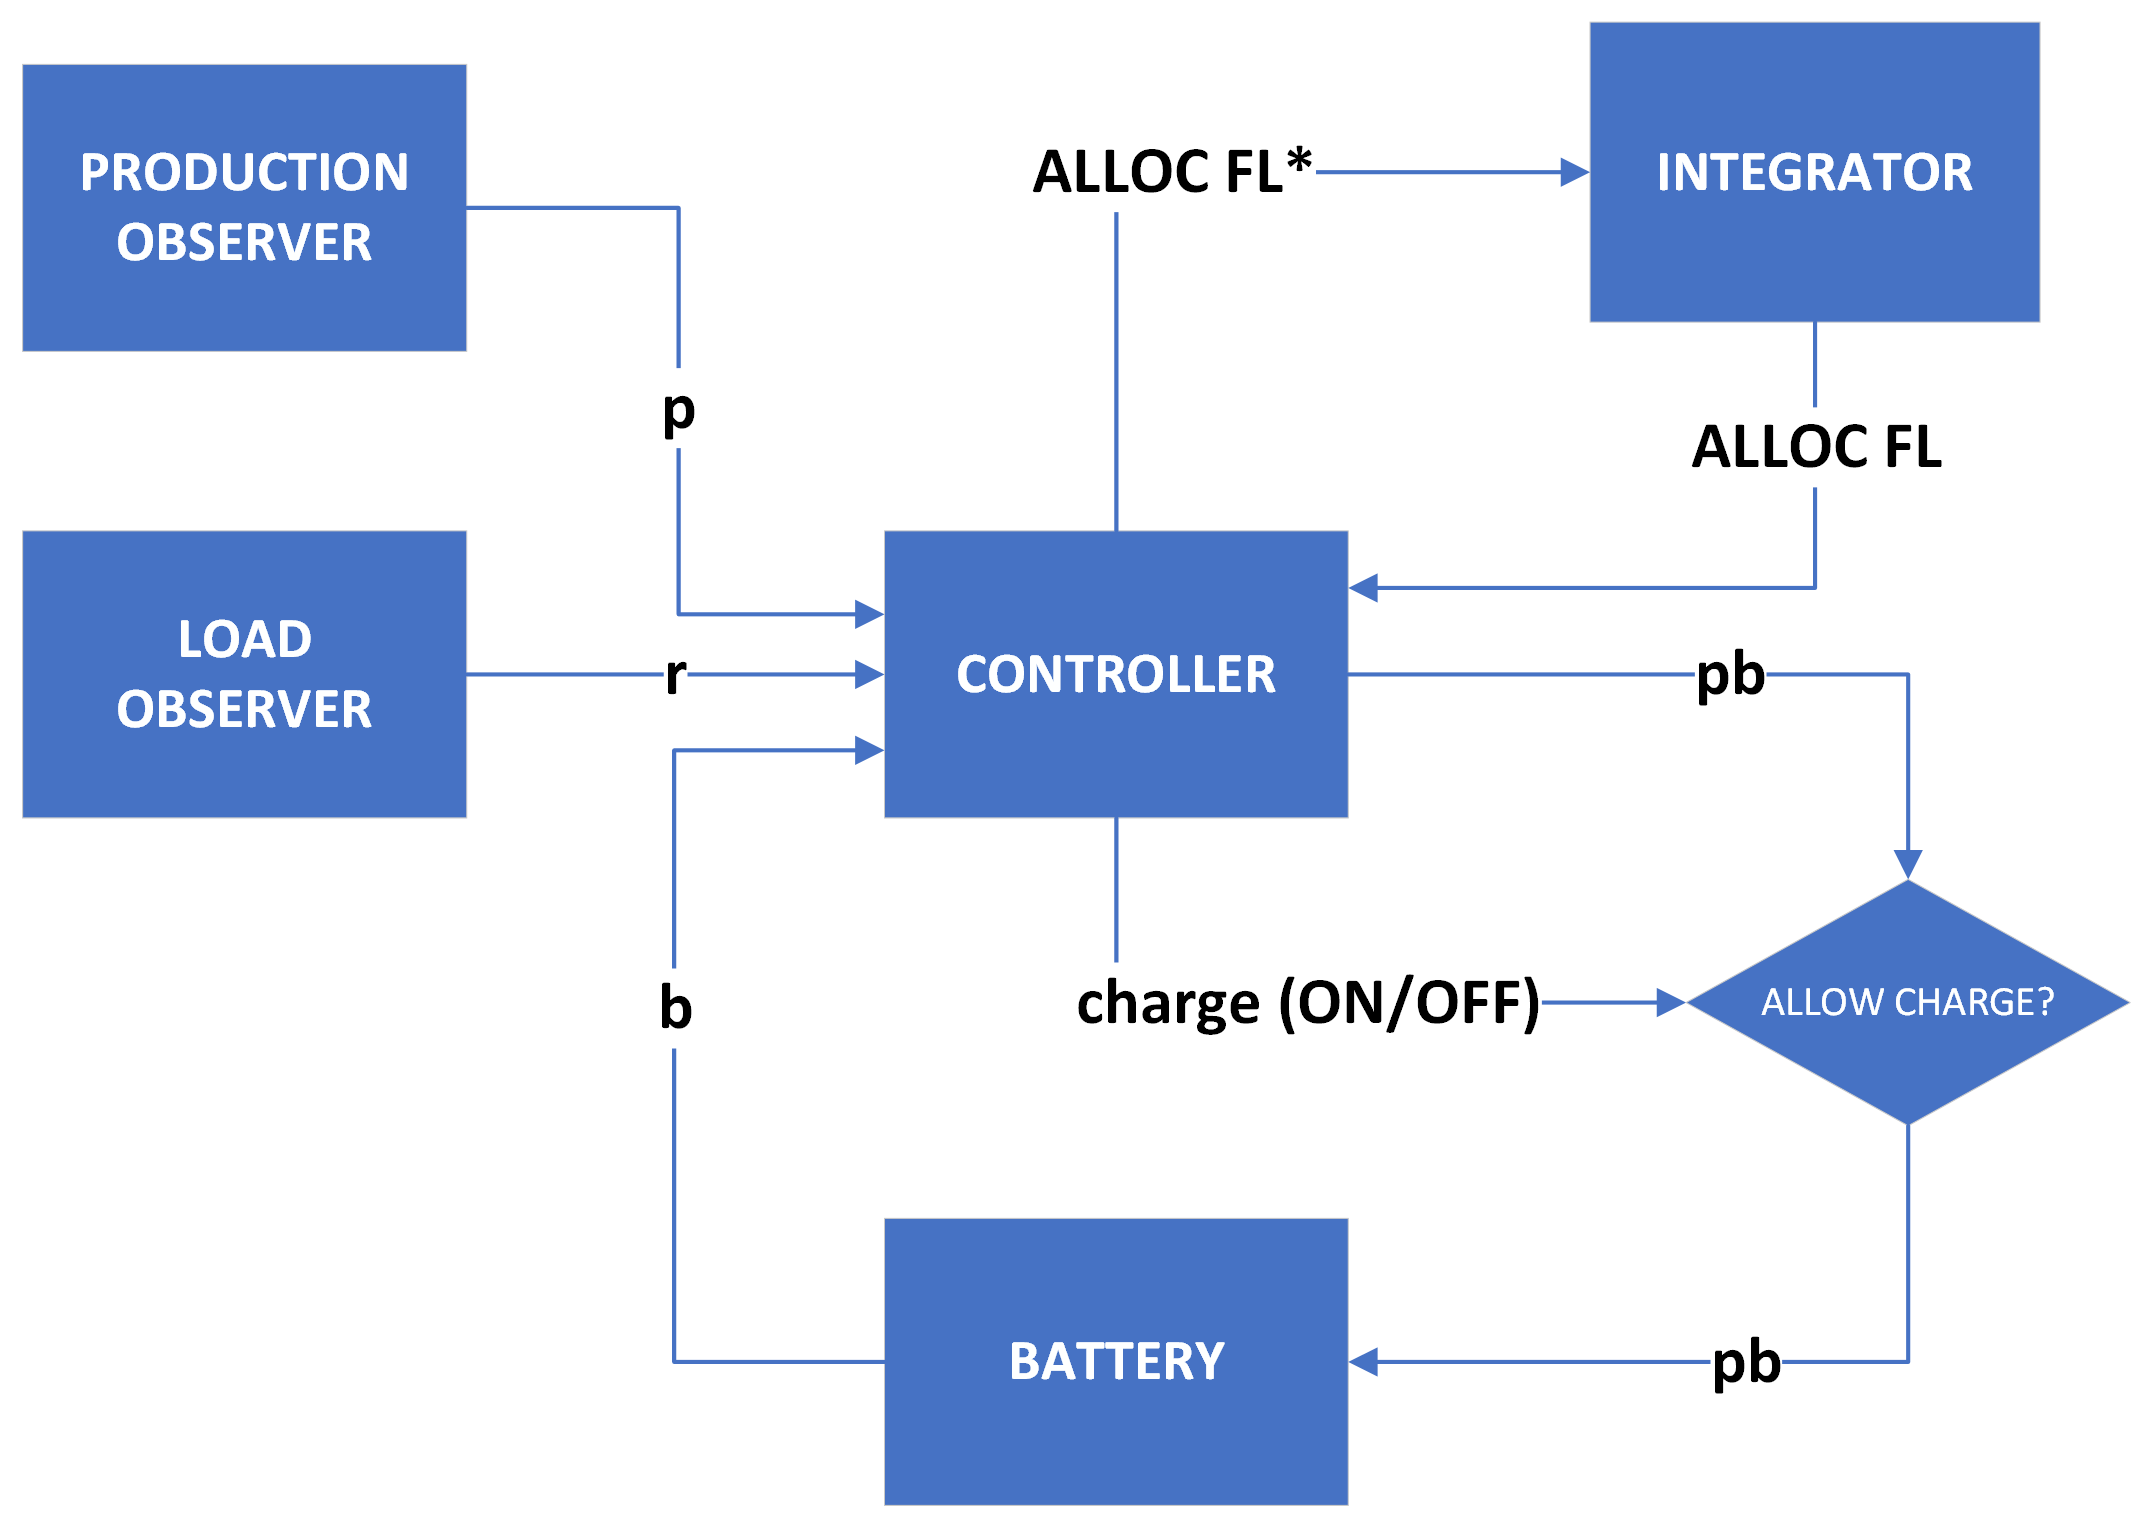
\includegraphics[width=\textwidth]{Figures/08Implementation/control_as_is_overview.png}
    \caption[Current control system block chart]{Chart showing the main components and signals of the current control system in simulation. $p$ - production at ts, $r$ - demand at ts, $b$ - battery capacity at ts, $pb$ - power to/from the battery, $charge(ON/OFF)$ - control signal to shut down battery charging. The $charge(ON/OFF)$ mechanism is highlighted in the battery control system shown in figure \ref{fig:current_battery_control_FSM}. The loop with ALLOC FL* and ALLOC FL through the integrator is to prevent the allocation to the flexible loads to exceed daily demand.}
    \label{fig:control_as_is_overview}
\end{figure}


\section{Battery Module}
The battery itself is simply modelled by an integrator integrating a saturated signal. The signal is saturated so that it cannot exceed the maximum charge/discharge rate of the battery. The integrator is also saturated to not exceed the max or min capacity of the battery. In addition, as the controller has a 15-min resolution, a block is added to convert this to hour resolution because the battery capacity is defined in watts per hour (W/h).

\begin{figure}
    \centering
    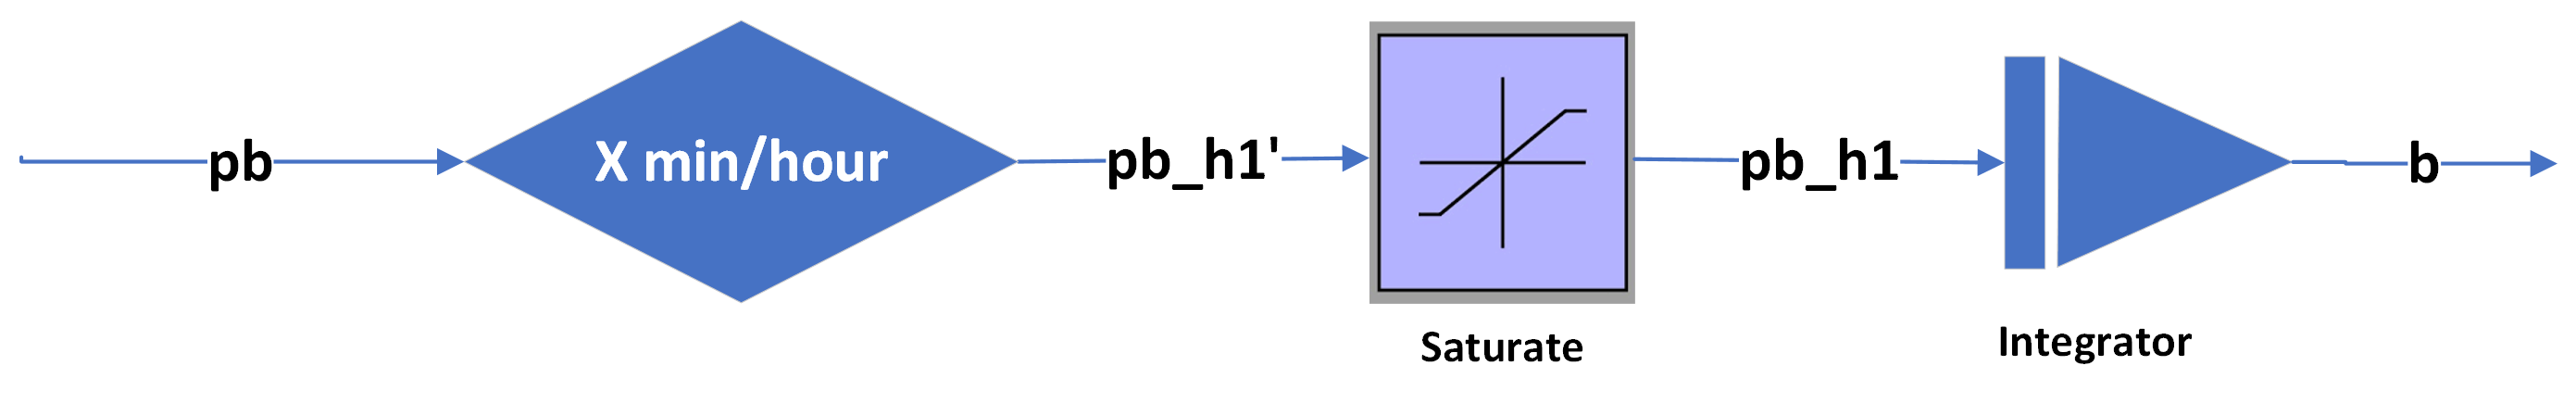
\includegraphics[width=\textwidth]{Figures/08Implementation/battery_model.png}
    \caption[Battery module block diagram]{Block diagram for the battery module. $p_b$ - power to/from the battery during the 15 min interval, $pb_{h1}'$ - power to/from the battery converted to hourly resolution, $pb_{h1}$ - is the same as $pb_{h1}'$ only saturated by the max charge/discharge rate.}
    \label{fig:battery_block}
\end{figure}

\section{Load Forecaster}

The load forecaster consist of the forecast block implementing the load forecasting algorithm outlined in section \ref{seq:load_forecasting}. This is wrapped in a feedback loop using a PID controller. A new forecast is made using the forecasting algorithm once every hour, the consumption is however measured every 15 minutes. In between the forecast the PID controller reduces the error between demand and the forecast until a new forecast is made. The algorithm shown in \ref{alg:load_forecast} shows the internal of the forecast block.

\begin{figure}
    \centering
    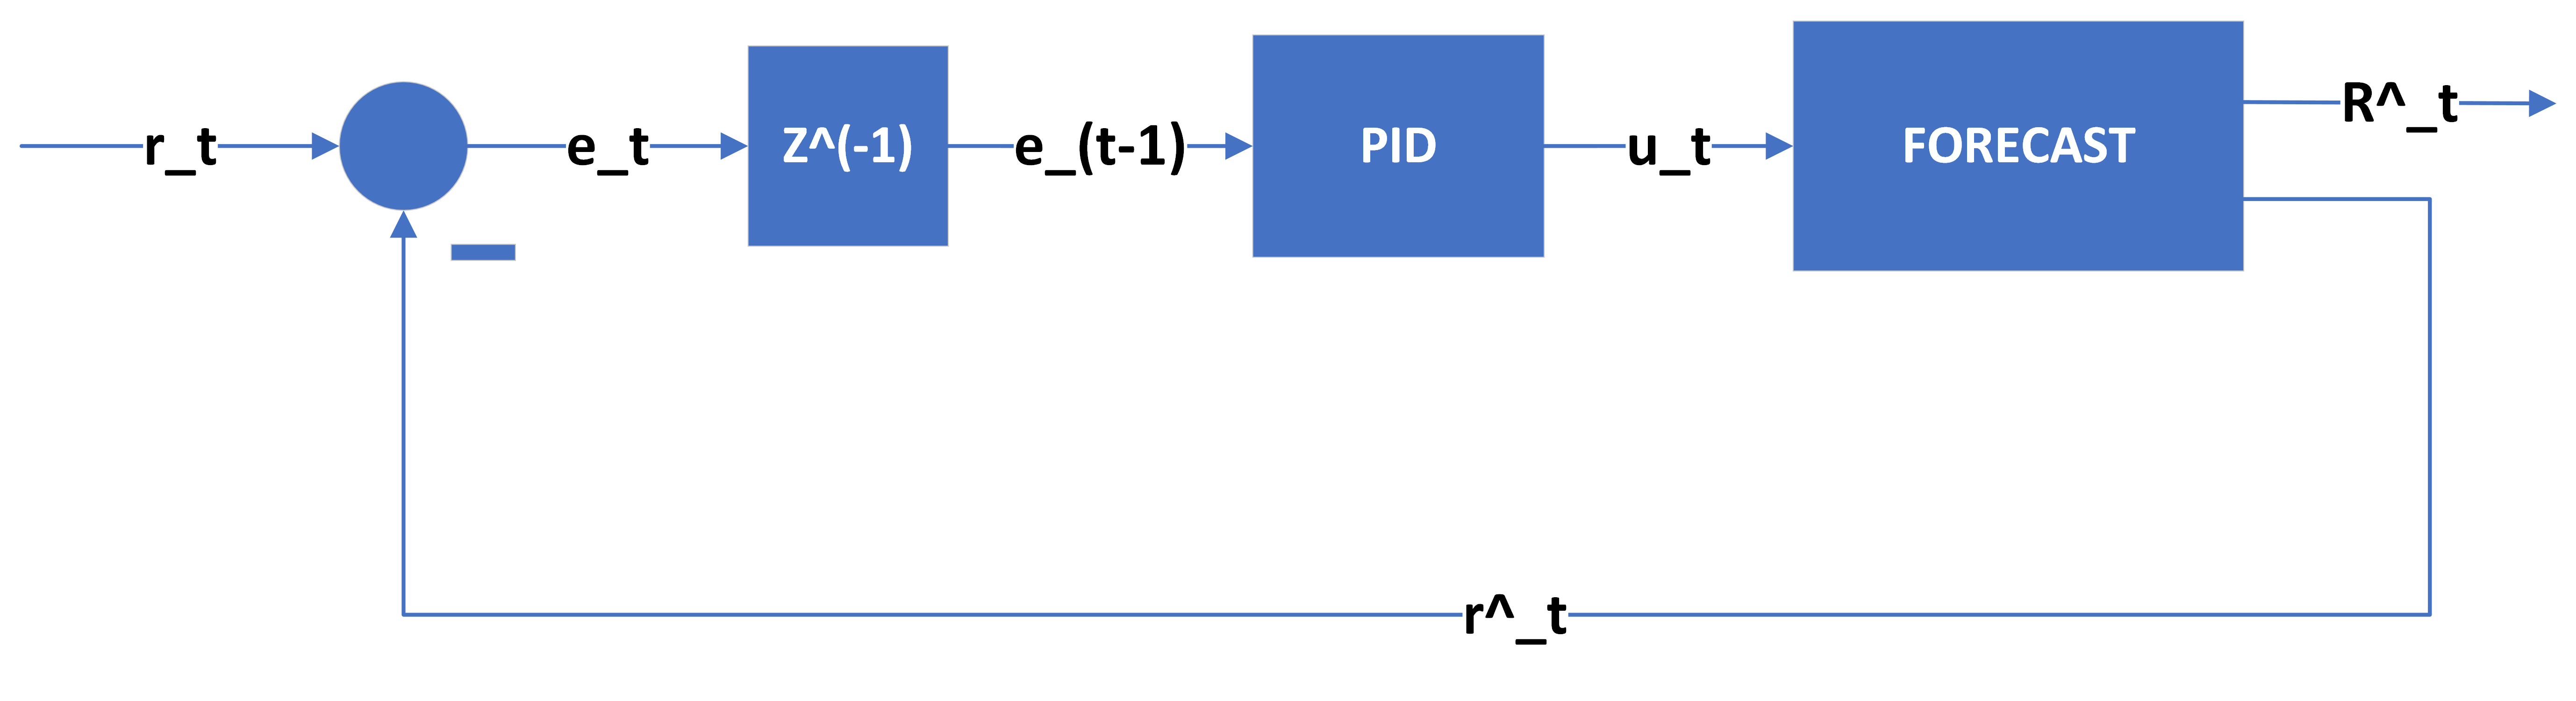
\includegraphics[width=\textwidth]{Figures/08Implementation/load_forecast.png}
    \caption[Load forecaster block diagram]{Block diagram for the load forecaster. $r_t$ - demand at time t, $\hat{r}_t$ - forecasted demand at time t, $e_t$ - estimation error at time t, $e_{t-1}$ - estimation error at time t-1, $u_t$ - forecast input at time t, $\hat{R}_t$ - forecasted demand over the whole prediction horizon at time t.}
    \label{fig:load_forecaster_block}
\end{figure}

\begin{algorithm}
\caption{Load forecaster algorithm}\label{alg:load_forecast}
\begin{algorithmic}
    \State$intitalize(historicData, coefficients,\hat{R}_0,predictionHorizon) $
    \State$r_t,u_t  \gets r_t, u_t $

\If{ts==hour}
    \State$historicData \gets [historicData,r_t]$
    \State$forecastData \gets arimaForecast(historicData,coefficients,predictionHorizon)$
\EndIf
    \State$\hat{R}_t = forecastData + u_t $
    \State$\hat{r}_t = \hat{R}_t(:,1)$
\end{algorithmic}
\end{algorithm}

\section{Production Forecaster}
The production forecaster has an identical internal layout to the forecast block. Also here the forecast algorithm from section \ref{seq:prod_forecasting} is wrapped in a feedback loop with an PID control to minimize error while until the next forecast is made. Algorithm \ref{alg:prod_forecast} shows the internal of the forecast block of the production forecaster module.

\begin{figure}
    \centering
    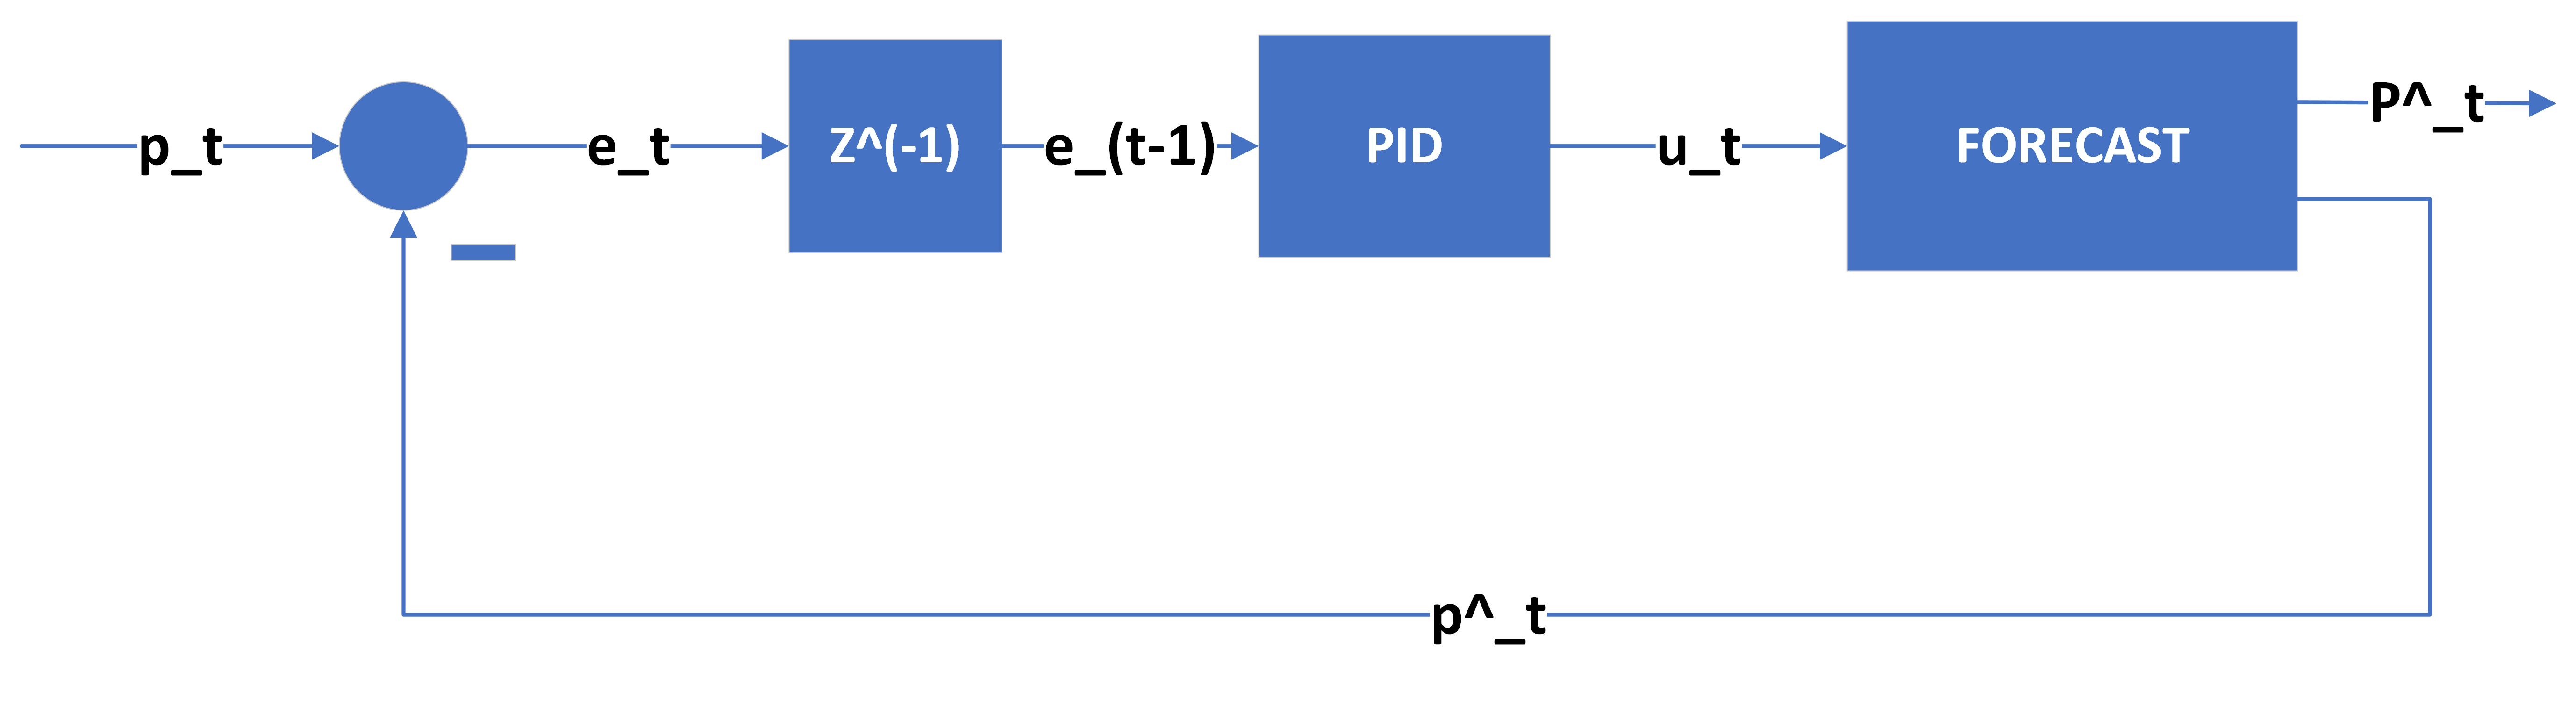
\includegraphics[width=\textwidth]{Figures/08Implementation/prod_forecast.png}
    \caption[Production forecaster block diagram]{Block diagram for the production forecaster. $p_t$ - demand at time t, $\hat{p}_t$ - forecasted demand at time t, $e_t$ - estimation error at time t, $e_{t-1}$ - estimation error at time t-1, $u_t$ - forecast input at time t, $\hat{P}_t$ - forecasted production over the whole prediction horizon at time t.}
    \label{fig:prod_forecaster_block}
\end{figure}

\begin{algorithm}
\caption{Production forecaster algorithm}\label{alg:prod_forecast}
\begin{algorithmic}
    \State$intitalize(historicData, coefficients,\hat{P}_0,predictionHorizon) $
    \State$p_t,u_t  \gets p_t, u_t $

\If{ts==hour}
    \State$historicData \gets [historicData,p_t]$
    \State$forecastData \gets modelForecast(historicData,coefficients,predictionHorizon)$
\EndIf
    \State$\hat{P}_t = forecastData + u_t $
    \State$\hat{r}_t = \hat{P}_t(:,1)$
\end{algorithmic}
\end{algorithm}



\section{Optimizer}
The optimizer implements the design from \ref{sec:optimization}. The optimizer algorithm including the non-linear optimization and post-processing is outlined in algorithm \ref{alg:optimizer}. The non-linear optimization is performed using Matlabs \textit{fmincon} with the 'interior-point' algorithm.

\begin{algorithm}
\caption{Optimizer algorithm}\label{alg:optimizer}
\begin{algorithmic}
    \State$\hat{R},\hat{P},b  \gets \hat{R}_t,\hat{P}_t,b_t$ 
    \State$C, K \gets C, K $
    
\If{ts==hour}
    \State$@(x)constraints \gets constraints(\hat{P},b)$
    \State$@(x)objectiveFunction \gets objectiveFunction(\hat{R},C,b,K)$
    \State$L^*,pb^* = optimize(objectiveFunction, constraints)$
    \State$allocNFL_{ts},allocFL_{ts} \gets splitFlexAndNonFlexLoads(L^*)$
    \\
    \State$priorityNFL_{ts} \gets allocNFL_{ts}\div\hat{R}(1:n_{NFL},1)$
    \State$priorityNFL,priorityIndex = sort(priorityNFL,descending)$

    \For{$\text{i in length}(allocFL_{ts})$}
        \State$flexLoad = allocFL_{ts}(i) $
        \If{$flexLoad \leq flexLoadMinW$}
            \State$allocFlexLoad(i) = flexLoad$
        \Else
            \State$allocFlexLoad(i) = 0$
        \EndIf
    \EndFor\\
    
    \State$pb \gets pb^*(1)$\\

    \State  $Out \gets priorityIndex,  allocFlexLoad,  pb$
\EndIf
\end{algorithmic}
\end{algorithm}

\section{Controller current control system}
The controller for the current control system includes both the controller itself and the integrator in figure \ref{fig:control_as_is_overview}. The integrator is included to stop the flexible loads from exceeding their demand. \ref{alg:current_control}

\begin{algorithm}
\caption{Current Control Algorithm}\label{alg:current_control}
    \begin{algorithmic}
        \State $\text{IN} \gets \text{\textit{inv\_max}, \textit{b\_min}, \textit{b\_max}, \textit{pb\_min}, \textit{pb\_max}}$ \Comment{Fetch Constants}
        \State $\text{IN} \gets \text{\textit{r}, \textit{p}, \textit{b}, \textit{time}}$   \Comment{Fetch signals}    
    
        \State $\text{p\_load} \gets p + \min([\text{pb\_max}, (b - \text{b\_min})])$
        \State $\text{p\_load} \gets \min([\text{inv\_max}, \text{p\_load}])$
    
        \For{$i \gets 1 \text{ to } (\text{length}(r) - n\_defer\_loads)$}
            \State $\text{add\_load} \gets r(i)$
            \State $\text{add\_load\_id} \gets i$
            \If{$(\text{p\_load} - \text{add\_load}) > 0$}
                \State $\text{load}(\text{add\_load\_id}) \gets \text{add\_load}$
                \State $\text{p\_load} \gets \text{p\_load} - \text{add\_load}$
            \EndIf
        \EndFor
    
        \For{flexible Loads $f$}
            \If{$\text{time} \in f\_run\_interval$}
                \State $\text{add\_load\_id} \gets f\_load$
                \If{$(\text{p\_load} - \text{add\_load}) > 0$}
                    \State $\text{load}(\text{add\_load\_id}) \gets \text{add\_load}$
                    \State $\text{p\_load} \gets \text{p\_load} - \text{add\_load}$
                \EndIf
            \EndIf
        \EndFor
        
        \If{$b \geq \text{b\_max} \times 0.9$ \textbf{and} $p > \text{p\_load}$ \textbf{and} $\text{mod}(ts, 24) < 15$}
            \State $\text{battery\_charge\_stop} \gets 0$
        \EndIf
        \State{Output $\gets \text{load}, \text{battery\_charge\_stop}$}
    \end{algorithmic}
\end{algorithm}


\section{Controller}
The controller in the proposed control system implements the first step of the plan from the optimizer. It is shown in algorithm \ref{alg:controller}.